% !Mode::"TeX:Utf-8"
\documentclass[winfonts,UTF8]{article}
%\documentclass[UTF8]{article}
\usepackage{amssymb}
%\usepackage{ctex}
\usepackage{amsmath}
\usepackage{listings}
\usepackage{graphicx}
%\usepackage[demo]{graphicx}

\usepackage{caption}
\usepackage{subcaption}

%\usepackage{subfig}
%\usepackage{subfigure}

\usepackage{algorithm}
\usepackage{algorithmic}
%\usepackage{epsfig,subfigure,epstopdf}
%\usepackage{tikz}

%\usepackage{CJK}

%\usepackage[pdftex]{hyperref}

\usepackage[colorlinks,linkcolor=red,anchorcolor=blue,citecolor=green]{hyperref}

\usepackage[top=1in, bottom=1in, left=1in, right=1in]{geometry}


\begin{document}

    \title{CS388 Natural Language Processing\\Homework 3: Active Learning for Statistical Parsing}
    %\centerline{\textbf{Homework 2: Part-of-Speech Tagging with HMMs and CRFs}}
    \author{Jianyu Huang}
    \maketitle

    
\section{Introduction}

We would like to get good performance using as few annotated examples as possible when learning PCFGs from data, since it is expensive to construct large training corpora like significant by human efforts. In this assignment we attempt to reduce annotation cost by adopting active learning for PCFG parsing, based on the experiment in  (Hwa, 2000) \cite{hwa2000sample}.

Active learning, in particular, \emph{sample selection}, requires that the learner itself select the examples for annotation from a large sample of initially unannotated data. The goal is to pick training examples wisely in order to minimize the amount of data that needs to be annotated to achieve a desired level of performance. For statistical parsing, a training instance is a sentence and the annotation is a parse tree supplied by a linguistic expert.

The simplest approach to select training examples is \emph{uncertainty sampling}. For statistical parsing, we use the following ways to measure the uncertainty in the automation of a sentence: sentence length, normalized probability of the top parse, and tree entropy using the top 10 PCFG parses.

Finally we compare the performance of active learning based on different uncertainty selection metrics with random selection of training examples and present corresponding learning curves.


\section{Implementation}
\begin{enumerate}

\item In the first step I create an initial training set, an "unlabeled" training pool for active learning, and a test set. To create the initial training set, extract the first 50 sentences from section 00. For the unlabeled training set, concatenate sections 01-03 of WSJ. So we get 4485 additional potential training sentences (approximately 100,000 words). For testing, use WSJ section 20. I write a \emph{preprocessing.java} file to do the preprocessing by combine several files into one file, and count on the sentence number.

\item A simple command line interface to the {\tt{LexicalizedParser}} is provided to support for active learning. I implement {\tt ActiveLearn.java} in two steps.
\begin{enumerate}
\item \textbf{Initializion} I build the TreeBank objects for training set, "unlabeled" training pool and a test set from files with {\tt maketreebank} function and transform TreeBank objects into memorybank objects because we can add/remove trees in memoryTreebank objects.

\item \textbf{Iterations}
Since we can add/remove trees in memoryTreebank, we don't need to write out the next training bank and candidate pool to new files for the next generation, since we can simply add the selected trees into the training set and mark them as selected in the candidate pool so that they will not be selected in the following iterations. Though this way, we can iterate several times within one java execution. In each iteration, we will do the following parts.
\begin{itemize}
\item Sort the trees in candidate pool by uncertainty selection metrics. If the selection metrics is random, we only need to shuffle the list. Otherwise, we calculate the string length, the normalized probability of the top parse, or the tree entropy using the top 10 PCFG parses as the {\tt Comparator} for the {\tt Collections.sort()} function.
\item Add the random or most uncertain sentences by the sorted order whose total word count approximates 1500 from candidate pool into the training set.
\item Train the parser with {\tt trainFromTreebank} API based on the data in the training set.
\item Evaluate the performance of PCFG parser with {\tt EvaluateTreebank:testOnTreebank} API on the test set.
\item Output the evaluation results for this iteration: iteration number, number of training words, PCFG F1 score.
\item Generate the candidate pool for the next iteration by removing those selected trees in this iteration.
\end{itemize}
\end{enumerate}

\item Collect enough data to plot a learning curve (F1 score versus number of training words) for each sample selection function.

\end{enumerate}

\section{Experiment}
\begin{enumerate}
\item
The results for random selection function and three uncertainty selection function (sentence length, normalized probability of the top parse, and tree entropy using the top 10 PCFG parses) are shown in Table~\ref{tab:res}. The corresponding learning curves are shown in Figure~\ref{fig:curve}.



\begin{table}[!htbp]
\centering
{\footnotesize
\begin{tabular}{c|c|c|c|c|c|c|c|c}
\hline 
 & \multicolumn{2}{|c|}{random} &  \multicolumn{2}{|c|}{strlen} & \multicolumn{2}{|c}{prob} & \multicolumn{2}{|c}{entropy} \\ 
 \cline{2-9}
 & \# training words & F1 score & \# training words & F1 score & \# training words & F1 score & \# training words & F1 score\\ 
\hline
1 & 1514 & 47.78 & 1537 & 45.38 & 1514 & 45.67 & 1530 & 45.31\\
\hline
2 & 3017 & 52.23 & 3011 & 55.69 & 3012 & 49.92 & 3047 & 56.34\\
\hline
3 & 4511 & 55.19 & 4509 & 59.27 & 4518 & 59.23 & 4542 & 54.39\\
\hline
4 & 6022 & 57.32 & 6022 & 57.18 & 6008 & 63.92 & 6007 & 62.70\\
\hline
5 & 7513 & 57.47 & 7532 & 56.62 & 7511 & 64.93 & 7500 & 60.81\\
\hline
6 & 9021 & 57.74 & 9038 & 61.06 & 9008 & 66.28 & 9006 & 61.60\\
\hline
7 & 10524 & 64.93 & 10536 & 61.54 & 10515 & 67.46 & 10541 & 64.40\\
\hline
8 & 12020 & 65.10 & 12040 & 62.58 & 12027 & 68.64 & 12037 & 66.48\\
\hline
9 & 13507 & 66.72 & 13504 & 65.45 & 13511 & 70.05 & 13515 & 67.74\\
\hline
10 & 15017 & 69.47 & 15017 & 68.14 & 15003 & 70.57 & 15033 & 69.79\\
\hline
11 & 16545 & 68.05 & 16501 & 67.91 & 16511 & 71.11 & 16534 & 71.07\\
\hline
12 & 18004 & 70.29 & 18032 & 71.40 & 18014 & 71.78 & 18026 & 70.99\\
\hline
13 & 19518 & 71.27 & 19528 & 71.96 & 19530 & 72.46 & 19538 & 72.30\\
\hline
14 & 21020 & 71.77 & 21016 & 71.89 & 21016 & 72.83 & 21013 & 71.38\\
\hline
15 & 22523 & 71.97 & 22528 & 72.44 & 22512 & 73.18 & 22500 & 73.14\\
\hline
16 & 24003 & 72.68 & 24008 & 72.68 & 24010 & 73.62 & 24026 & 73.40\\
\hline
17 & 25509 & 72.66 & 25528 & 72.94 & 25509 & 73.89 & 25507 & 73.06\\
\hline
18 & 27021 & 72.99 & 27004 & 72.30 & 27032 & 73.40 & 27024 & 73.40\\
\hline
19 & 28512 & 74.90 & 28518 & 72.63 & 28509 & 74.49 & 28518 & 74.22\\
\hline
20 & 30023 & 75.04 & 30023 & 73.04 & 30035 & 73.85 & 30011 & 73.87\\
\hline
\end{tabular} 
}
\caption{Results of random selection function and three uncertainty selection function (sentence length, normalized probability of the top parse, and tree entropy using the top 10 PCFG parses)}
\label{tab:res}
\end{table}


\begin{figure}[!htbp]
\centering
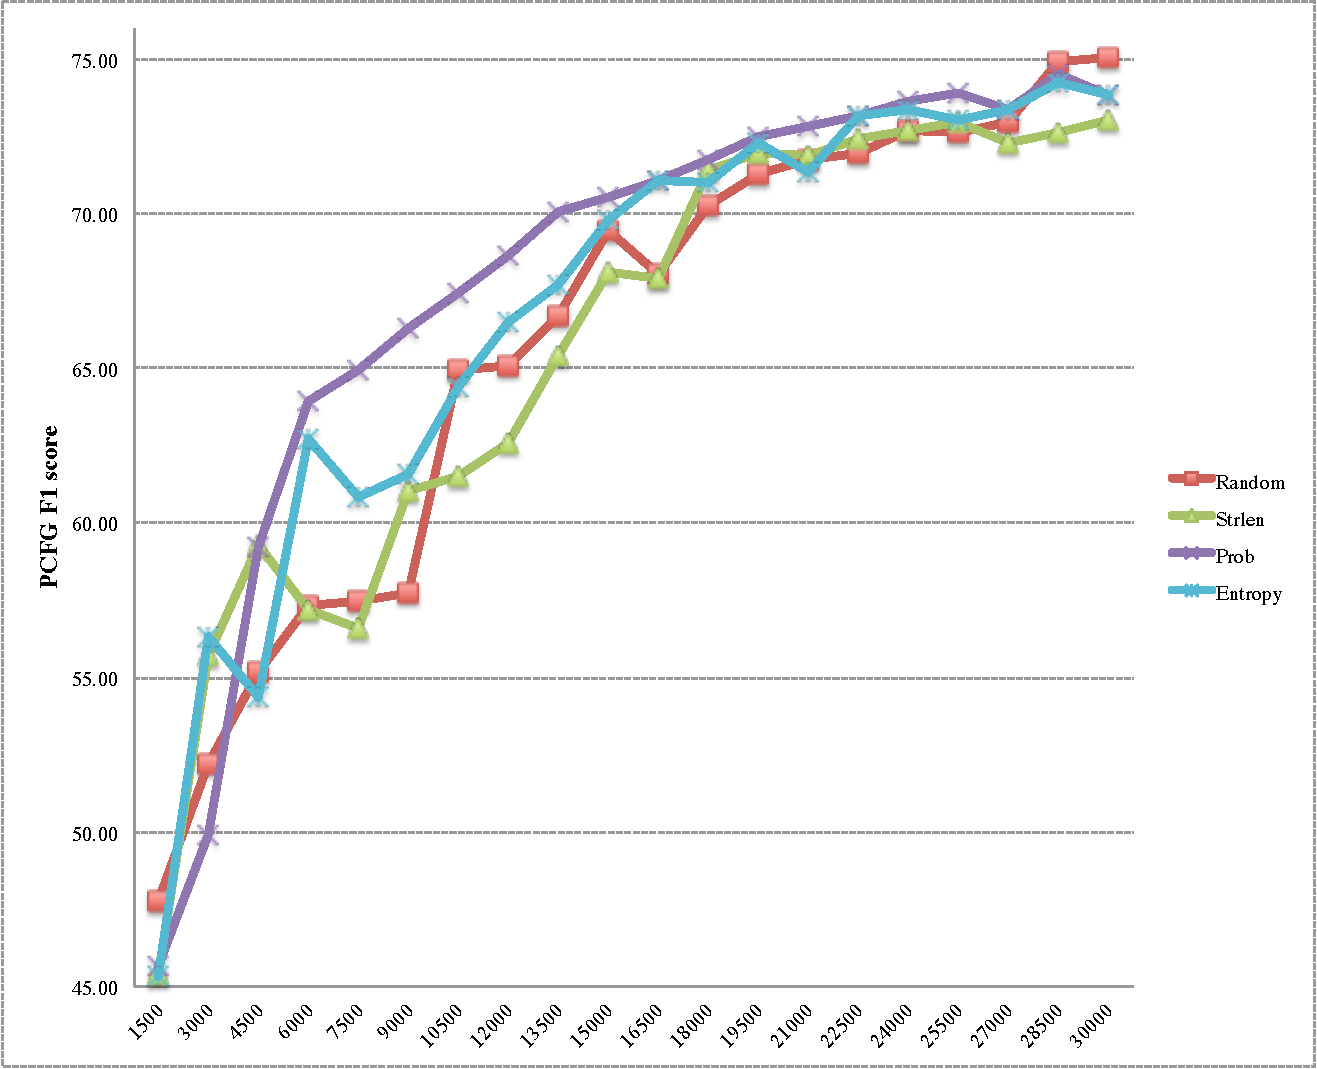
\includegraphics[width=0.6\textwidth]{res1.pdf}
\caption{Learning curves for different selection functions}
\label{fig:curve}
\end{figure}




%\begin{figure}[!htbp]
%\centering
%\addtocounter{subfigure}{-2}
%\begin{subfigure}[]{0.8\textwidth}
%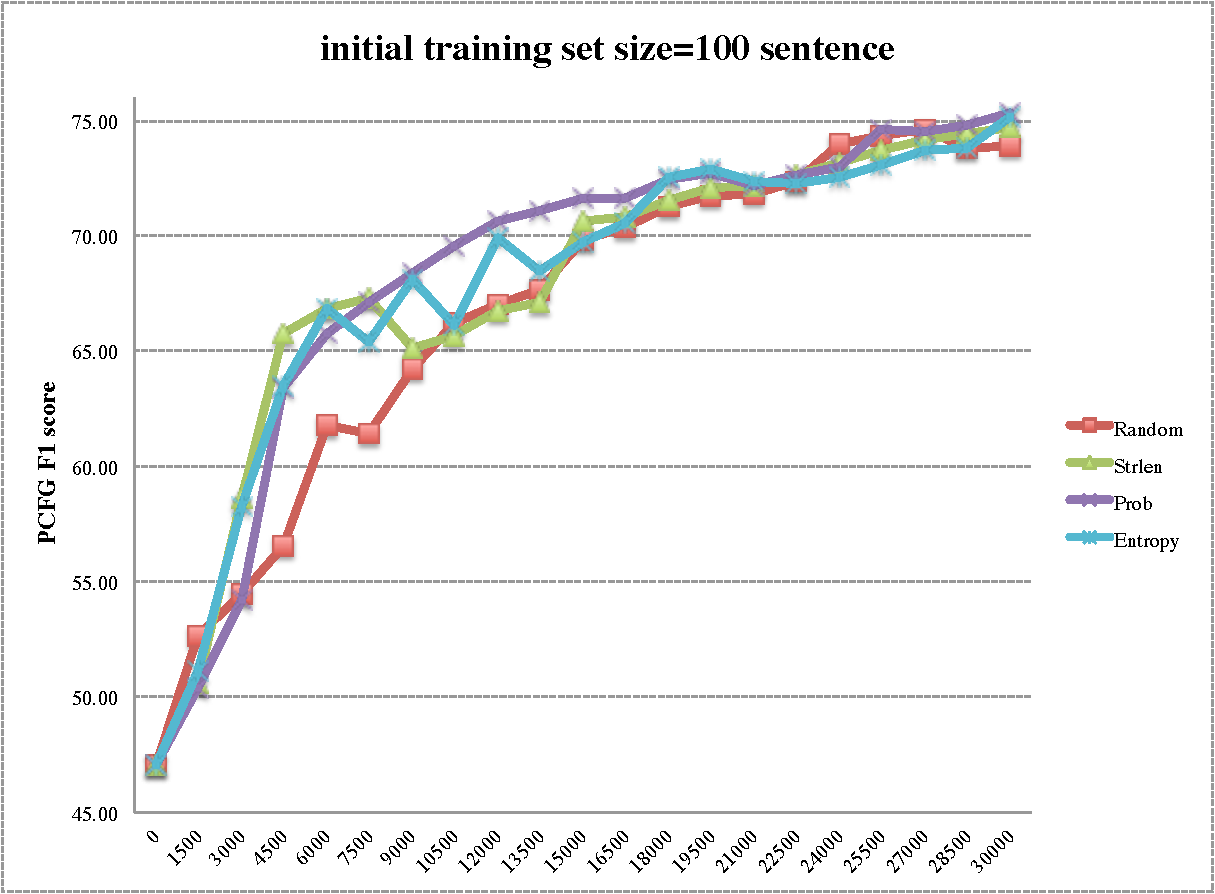
\includegraphics[width=\textwidth]{res3.pdf}
%\caption{atis}
%\label{fig:feature_atis}
%\end{subfigure}
%~
%\begin{subfigure}[]{0.8\textwidth}
%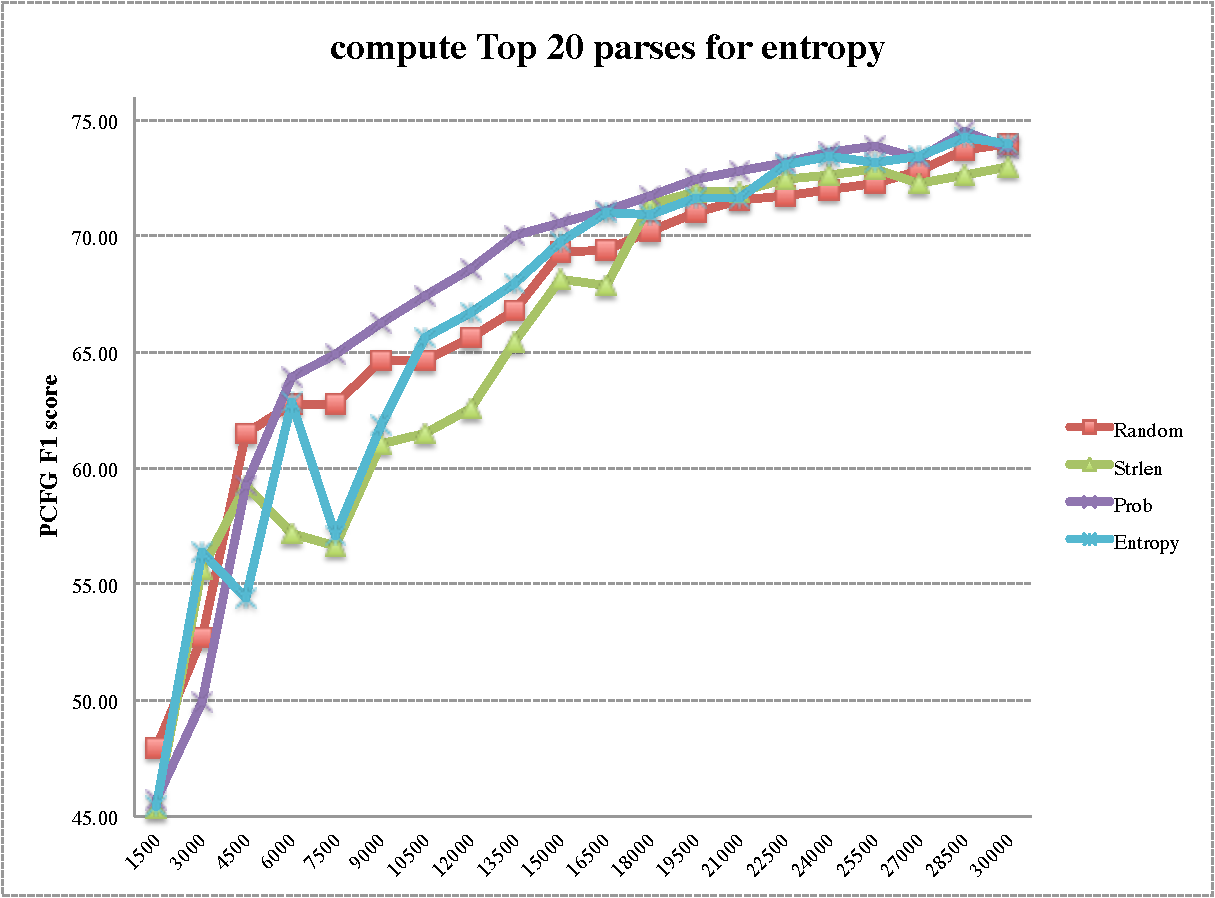
\includegraphics[width=\textwidth]{res4.pdf}
%\caption{wsj}
%\label{fig:feature_wsj}
%\end{subfigure}
%\caption{Results of adding extra orthographic features to CRF model on \emph{atis} and \emph{wsj} dataset}
%\label{fig:feature}
%\end{figure}

\item
In addition to the basic experiment, I also finish some extension experiments by changing the batch size of word count totals, changing the initial training set size, changing the Top K parses in Tree entropy, and changing the maximum iteration for each sampling function. The corresponding learning curves are shown in Figure~\ref{fig:res}.

\begin{enumerate}
\item Changing the batch size for word count totals.\\
Set  word count = 500.\\
\textbf{Observation}: When the batch size is in finer granularity, active learning method has obvious better learning rate than random selection in the beginning of the learning curve.
\item Changing the initial training set size.\\
There are 100 sentences from section 00 in the training set.\\
\textbf{Observation}: When the initial training set is larger, active learning will have more confidence on some examples, so it can figure out the relatively uncertain examples more confidently and ask the expert to annotate it, thus it will learn faster.
\item Changing the Top K parses in Tree entropy.\\
Compute the top 20 parses.\\
\textbf{Observation}: it will work slightly better to compute the top 20 parses for entropy than to compute 10 parses.
\item Changing the maximum iteration for each sampling function.\\
Set iteration = 40.\\
\textbf{Observation}: In the end of the learning curve, both active learning and random selection converges to a constant, since the information it can learn from the candidate pool becomes saturated.
\end{enumerate}
\begin{figure}[!htbp]
%\centering
\begin{subfigure}[b]{0.45\textwidth}
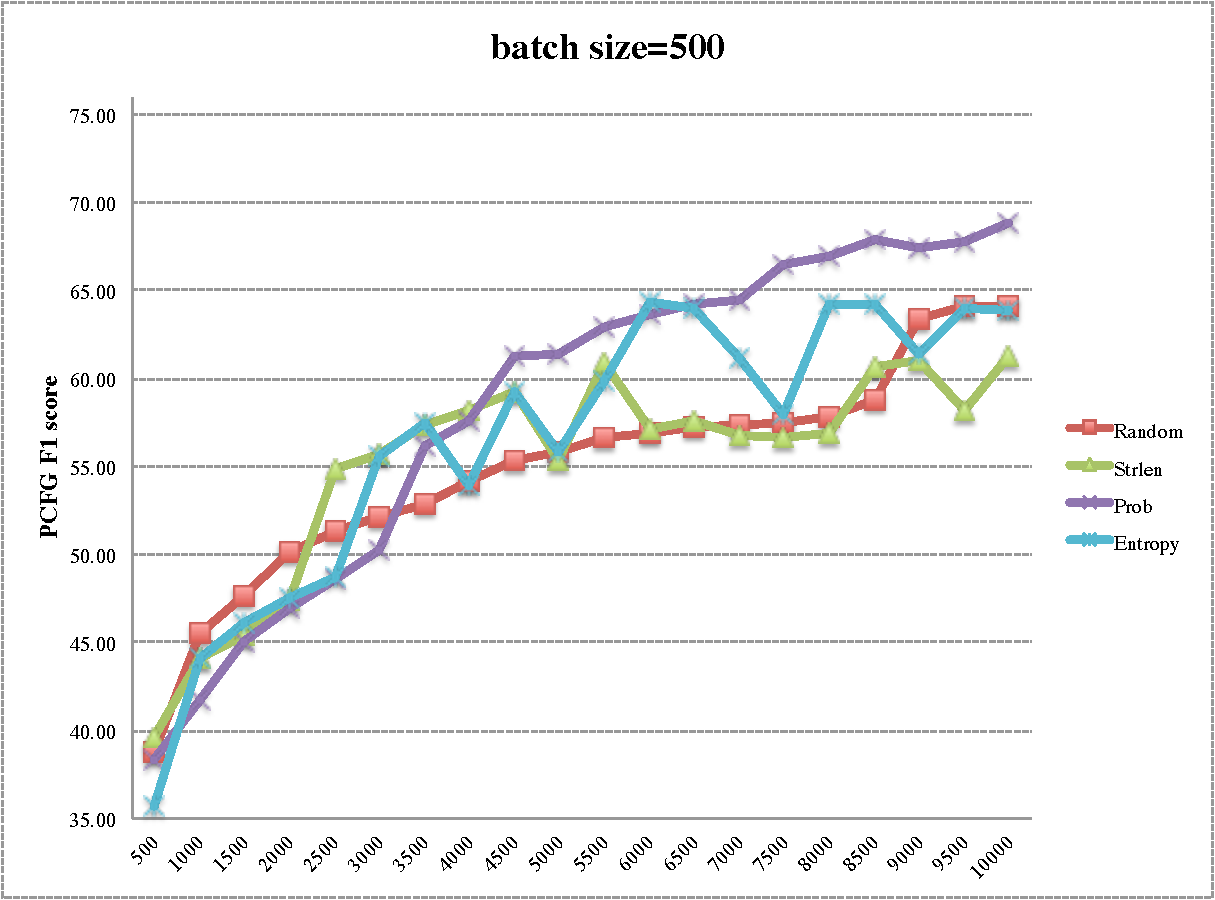
\includegraphics[width=\textwidth]{res2.pdf}
\caption{Changing the batch size for word count totals}
\label{fig:res_ext1}
\end{subfigure}
~
\begin{subfigure}[b]{0.45\textwidth}
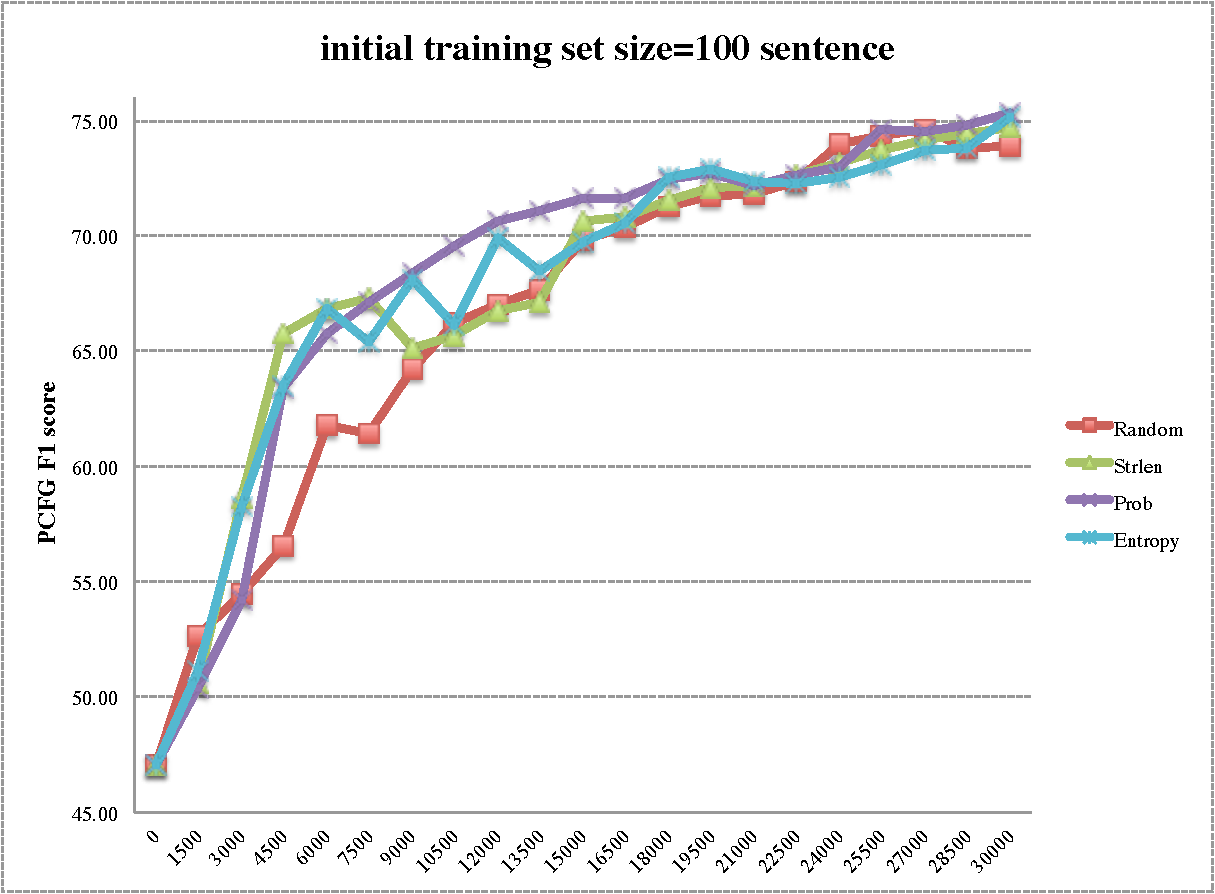
\includegraphics[width=\textwidth]{res3.pdf}
\caption{Changing the initial training set size}
\label{fig:res_ext2}
\end{subfigure}
~
\begin{subfigure}[b]{0.45\textwidth}
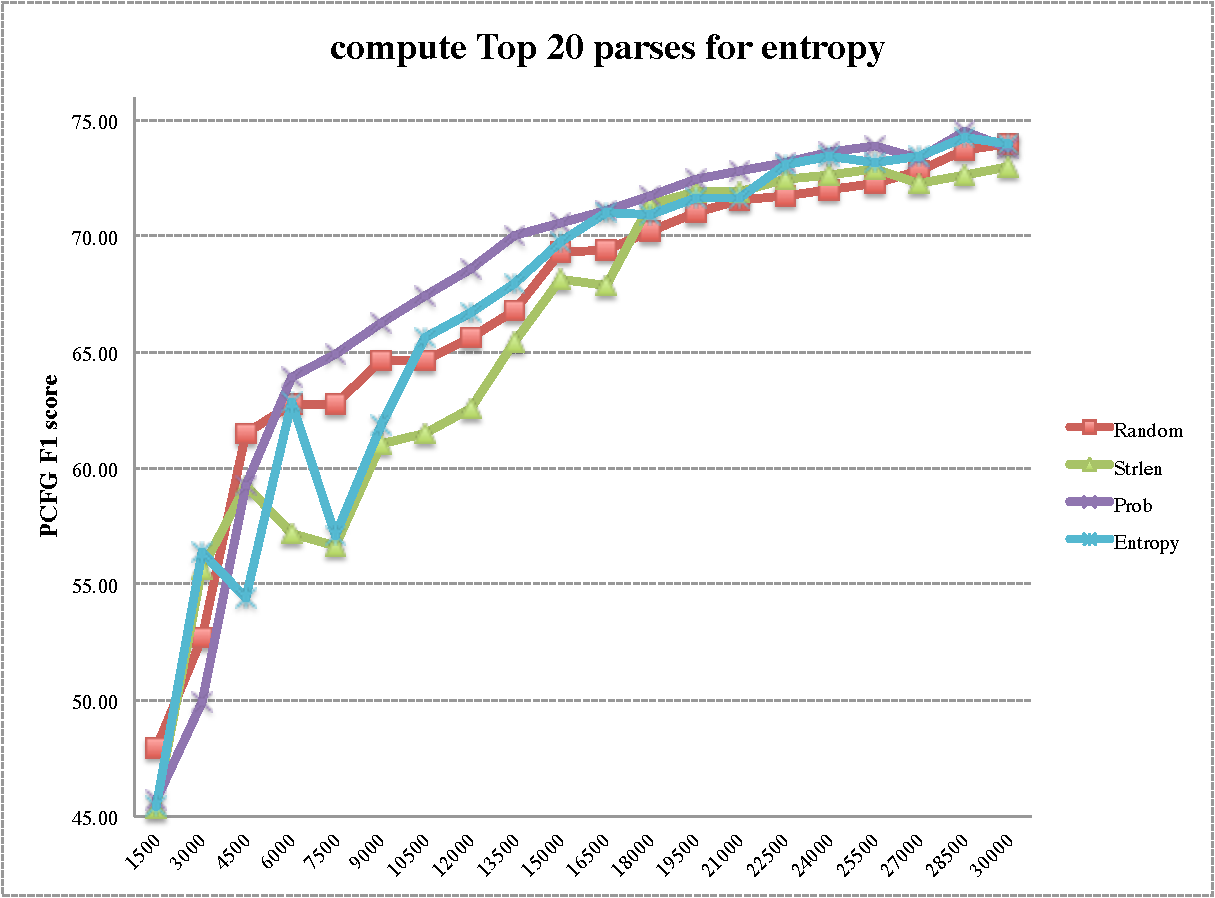
\includegraphics[width=\textwidth]{res4.pdf}
\caption{Changing the Top K parses in Tree entropy}
\label{fig:res_ext3}
\end{subfigure}
~~~~~~~~~~~~
\begin{subfigure}[b]{0.45\textwidth}
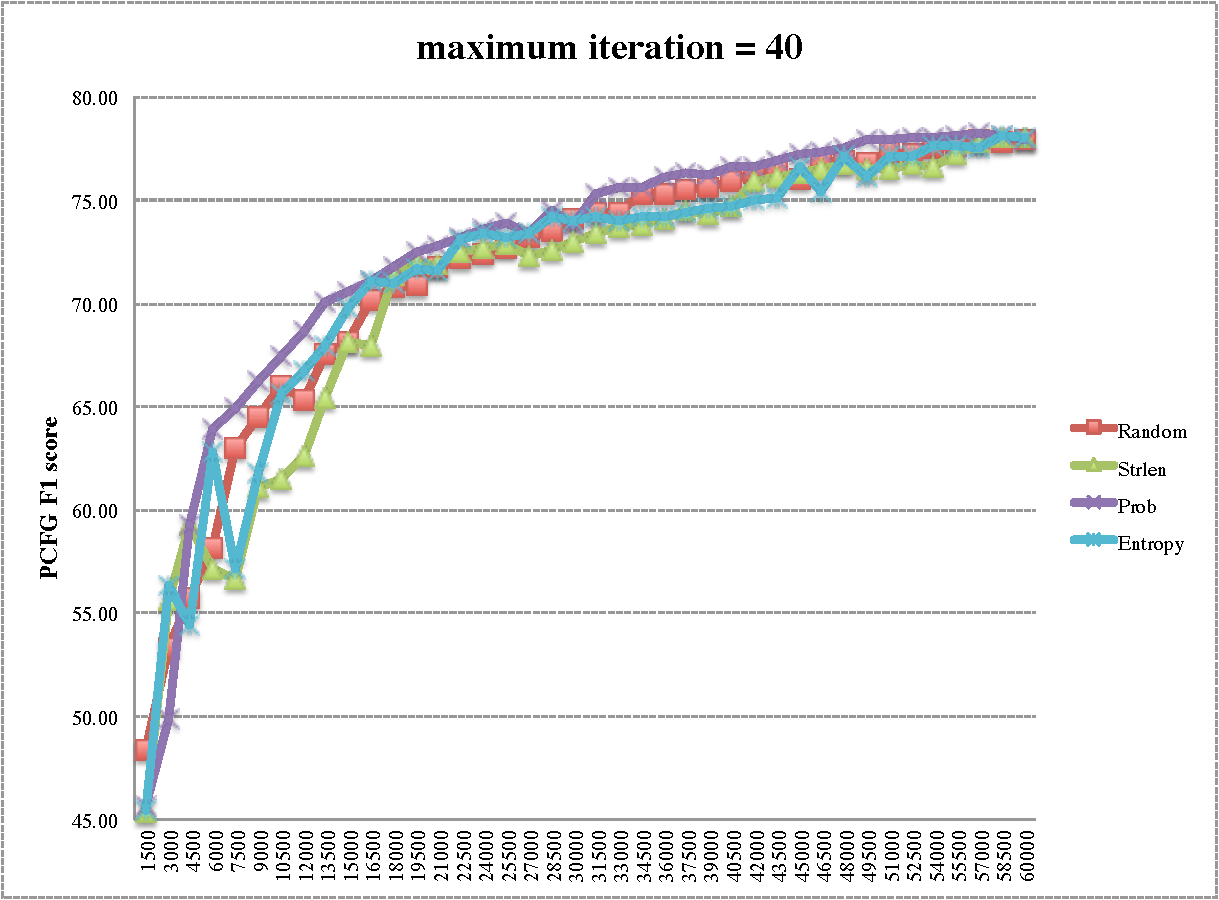
\includegraphics[width=\textwidth]{res5.pdf}
\caption{Changing the maximum iteration}
\label{fig:res_ext3}
\end{subfigure}
\caption{Extension Experiments}
\label{fig:res}
\end{figure}


\end{enumerate}
\section{Discussion}
\subsection{Comparison between Active Learning and Random Selection}
\begin{enumerate}
\item Active learning methods perform better than random selection of training examples.
There are several reasons: \\
\begin{itemize}
\item Active learning selects a small batch of the most useful examples for annotation and asks the expert to annotate them. By obtaining feedback on the cases in which it is most uncertain, it hopes to learn more than obtaining labels on random sentences in which its existing model is perhaps already quite confident in, and from which it would therefore not learn much.
\item Random selection just selects the random examples, so the "learning rate" is always the same. It cannot distinguish the examples which it can learn more and the examples it cannot learn much, since there are some examples it is quite confident in.
\end{itemize}
\item Active learning performs best in the beginning and middle part of the learning curve.
\begin{itemize}
\item In the initial and the middle parts of the learning curve, active learning method selects the most useful examples for annotation by obtaining feedback on the cases in which it is most uncertain, so it will always learn faster than random selection. So the learning rate of active learning method is faster than random selection in the initialization part.

\item However, in the final part of the learning curve, the learning curves of both active learning and random selection converges to a constant, since the information it can learn from the candidate pool becomes saturated. We notice that finally random selection may perform slightly better than active learning, because there is no discrimination in its selection of examples.
\end{itemize}
\end{enumerate}
\subsection{Comparison between Different Uncertainty Metrics}
\begin{enumerate}
\item Measuring the uncertainty by normalized probability of the top parse works best.
\begin{itemize}
%Observed Difference between methods\\
\item We observe that all three uncertainty selection functions work well when the number of training words is small than 6000, but it may be unstable in some data points. Measuring the uncertainty by normalized probability of the top parse works better than by tree entropy using the top 10 PCFG parses, while tree entropy using the top 10 PCFG parses works better than sentence length.
%\begin{itemize}
\item Uncertainty measured by the normalized probability of the top parse improves the learning rate, since the normalized probability reflects the confidence of the model in the testing set most accurately.
\item Entropy reflects the disorder of the parses, so it will also reflects the uncertainty.
\item While the simplistic sentence length selection function is less helpful, its learning rate still improves slightly faster than the random selection baseline, since longer sentences are clearly more difficult for a human to annotate, thus more uncertain.
%\end{itemize}
\end{itemize}
\item Compare results with \cite{hwa2000sample}.
\begin{itemize}
\item In general, the performance of tree entropy using the top 10 PCFG parses and sentence length matches the result of \cite{hwa2000sample}, although my result is unstable in some data points. This is because the data distribution of unlabeled training set.
\item \cite{hwa2000sample} doesn't measure the uncertainty with normalized probability of the top parse.
\end{itemize}
\end{enumerate}
\section{Conclusion}
Through this assignment, We reduce annotation cost by adopting active learning for PCFG statistical parsing. It turns out that active learning performs better than random selection of training examples. Among the three uncertainty selection functions, normalized probability of the top parse works the best.
\section{Apendix} \label{appendix}
%\subsection{Extension Experiments}


%\subsection{Testing result}
To create the initial training set, extract the first 50 sentences from section 00. For the unlabeled training set, concatenate sections 01-03 of \emph{WSJ}. So we get 4485 additional potential training sentences (approximately 100,000 words). For testing, use \emph{WSJ} section 20. All the results are stored in "hw3.xlsx" file. Note that for single-word sentences, I don't normalize the probability by sentence minus 1, since it will lead to infinite.


%\cite{hwa2000sample}.

\section{Reference}
\renewcommand\refname{\vskip -0.25cm}
\refname
\bibliographystyle{plain}
\bibliography{hw3}



\end{document} 
















